\documentclass[11pt,letterpaper]{article}
\usepackage[T1]{fontenc}
\usepackage[utf8]{inputenc}
\usepackage{mathptmx}
\usepackage[margin=2.2cm]{geometry}
\usepackage{graphicx,xcolor,booktabs,amsmath,amssymb,siunitx,tikz,caption,subcaption,hyperref,fancyhdr,listings}
\lstset{language=Python,columns=fullflexible,keepspaces=true,basicstyle=\ttfamily\scriptsize,keywordstyle=\color{blue!60!black}\bfseries,commentstyle=\color{green!40!black}\itshape,stringstyle=\color{red!50!black},numbers=left,numberstyle=\tiny\color{gray},frame=single,breaklines=true,showstringspaces=false,backgroundcolor=\color{gray!5},inputencoding=utf8,extendedchars=true,literate={á}{{\'a}}1 {é}{{\'e}}1 {í}{{\'i}}1 {ó}{{\'o}}1 {ú}{{\'u}}1 {ñ}{{\~n}}1 {°}{{$^\circ$}}1 {σ}{{$\sigma$}}1 {Δ}{{$\Delta$}}1 {≈}{{$\approx$}}1 {·}{{$\cdot$}}1 {±}{{$\pm$}}1}
\renewcommand{\lstlistingname}{Código}
\hypersetup{colorlinks=true,linkcolor=blue!50!black,citecolor=blue!50!black,urlcolor=blue!50!black}
\renewcommand{\figurename}{Figura}\renewcommand{\tablename}{Tabla}\renewcommand{\refname}{Referencias}\renewcommand{\abstractname}{Resumen}
\captionsetup{font=small,labelfont=bf}
\pagestyle{fancy}\fancyhf{}\lhead{\small Concentración de esfuerzos en placa con agujero}\rhead{\small Ing. Juan Diego Rubio Ruiz}\cfoot{\thepage}
\title{\textbf{Concentración de esfuerzos en una placa con agujero a tensión:\\ análisis por elemento finito, convergencia de malla y validación analítica}}
\author{Ing. Juan Diego Rubio Ruiz\\\small Maestría en Ciencias en Ingeniería Física, UMSNH}
\date{Octubre de 2026}
\begin{document}
\maketitle
\begin{abstract}
Se calculó el esfuerzo máximo en una placa de acero de ancho finito ($d/W=0.2$) con un agujero central, sometida a tensión uniaxial de \SI{10}{MPa}, mediante un modelo 2D de esfuerzo plano en Ansys Mechanical 2026 R1 con elementos cuadriláteros cuadráticos y doble simetría. Un estudio de convergencia con cinco mallas (\num{1035} a \num{59977} nodos) da $\sigma_{x,\max}=\SI{31.52}{MPa}$ en la malla más fina y un valor extrapolado de Richardson de \SI{31.59}{MPa}, con un índice de convergencia de malla (GCI) de \SI{0.27}{\%}. El resultado queda a \SI{0.6}{\%} de la estimación empírica de Heywood (\SI{31.4}{MPa}), dentro de la incertidumbre propia de esa fórmula, y el perfil de esfuerzos en la sección neta reproduce la forma de la solución de Kirsch con las desviaciones esperadas por el ancho finito. El equilibrio de la sección neta se verificó con un error menor a \SI{0.001}{\%}. La solución analítica, el post-procesamiento y las gráficas se automatizaron en Python (Apéndice~\ref{ap:codigo}).
\end{abstract}

\section{Planteamiento}
Una placa de longitud $L=\SI{200}{mm}$, ancho $W=\SI{100}{mm}$ y espesor $t=\SI{5}{mm}$ tiene un agujero central de diámetro $d=2a=\SI{20}{mm}$. Sus extremos están sometidos a un esfuerzo uniforme de tensión $\sigma=\SI{10}{MPa}$ en dirección $x$. El material es acero estructural lineal elástico e isótropo ($E=\SI{200}{GPa}$, $\nu=0.3$). Interesa el esfuerzo máximo, que aparece en el borde del agujero sobre el eje transversal a la carga ($\theta=\SI{90}{\degree}$), y el factor de concentración de esfuerzos.

\subsection{Solución de Kirsch (placa infinita)}
Para una placa infinita con un agujero circular de radio $a$ bajo tensión remota $\sigma$, la solución clásica de Kirsch da el esfuerzo tangencial
\begin{equation}
\sigma_{\theta\theta}(r,\theta)=\frac{\sigma}{2}\left(1+\frac{a^2}{r^2}\right)-\frac{\sigma}{2}\left(1+\frac{3a^4}{r^4}\right)\cos 2\theta .
\end{equation}
Sobre la línea $\theta=\pi/2$ (el eje $y$, donde $x=0$ y $r=y$) se tiene $\cos 2\theta=\cos\pi=-1$ y $\sigma_{\theta\theta}=\sigma_x$, de modo que
\begin{equation}
\sigma_x(0,y)=\frac{\sigma}{2}\left(2+\frac{a^2}{y^2}+\frac{3a^4}{y^4}\right)=\sigma\left(1+\frac{1}{2}\frac{a^2}{y^2}+\frac{3}{2}\frac{a^4}{y^4}\right),\qquad y\ge a .
\label{eq:kirsch}
\end{equation}
En el borde del agujero ($y=a$), $\sigma_x=\sigma(1+\tfrac12+\tfrac32)=3\sigma=\SI{30}{MPa}$: el factor de concentración de la placa infinita es $K_t=3$. Lejos del agujero, $\sigma_x\to\sigma$.

\subsection{Corrección por ancho finito (Heywood)}
En una placa de ancho finito el material retirado por el agujero obliga a que la carga pase por una sección neta menor. Se define el esfuerzo nominal neto
\begin{equation}
\sigma_{\text{nom}}=\frac{\sigma W t}{(W-d)\,t}=\frac{\sigma}{1-d/W}=\frac{10}{1-0.2}=\SI{12.5}{MPa},
\end{equation}
y la aproximación de Heywood para el factor de concentración referido a la sección neta,
\begin{equation}
K_{t,n}=2+\left(1-\frac{d}{W}\right)^3=2+0.8^3=2.512 .
\end{equation}
Así, $\sigma_{\max}=K_{t,n}\,\sigma_{\text{nom}}=2.512\times12.5=\SI{31.40}{MPa}$, equivalente a un factor bruto $K_{t,g}=\sigma_{\max}/\sigma=3.14$. La fórmula de Heywood es un ajuste empírico con una precisión del orden de \SI{1}{\%} \cite{pilkey}, de modo que define una banda de referencia y no un valor exacto.

\section{Modelo de elemento finito}
\begin{figure}[h]
\centering
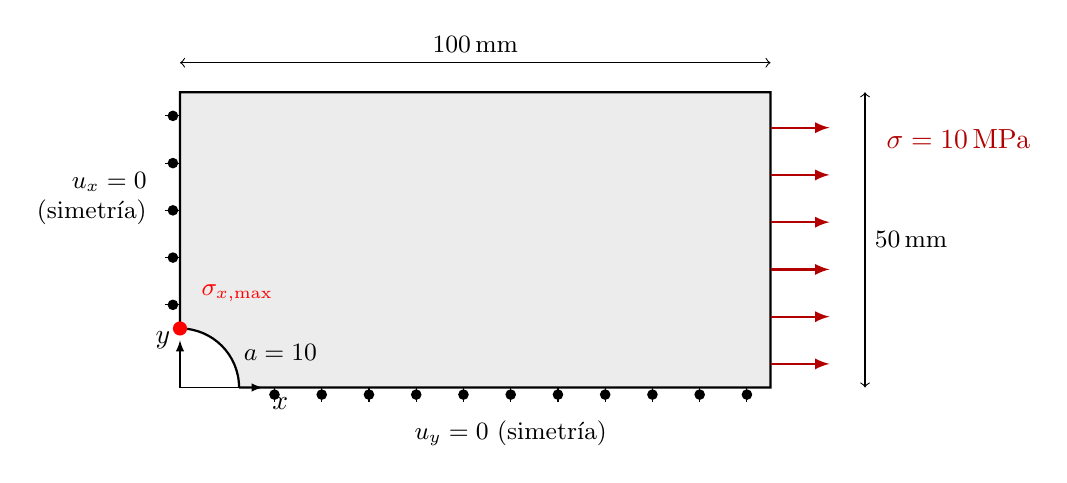
\begin{tikzpicture}[scale=0.075]
\fill[gray!15] (10,0) -- (100,0) -- (100,50) -- (0,50) -- (0,10) arc (90:0:10) -- cycle;
\draw[thick] (10,0) -- (100,0) -- (100,50) -- (0,50) -- (0,10) arc (90:0:10);
\foreach \y in {14,22,...,50} {\draw (0,\y) -- (-2.5,\y); \fill (-1.2,\y) circle (0.9);}
\foreach \x in {16,24,...,96} {\draw (\x,0) -- (\x,-2.5); \fill (\x,-1.2) circle (0.9);}
\foreach \y in {4,12,...,48} {\draw[-latex,thick,red!70!black] (100,\y) -- (110,\y);}
\node[right,red!70!black] at (118,42) {$\sigma=\SI{10}{MPa}$};
\node[left,align=right,font=\small] at (-4,32) {$u_x=0$\\(simetría)};
\node[below,font=\small] at (56,-4) {$u_y=0$ (simetría)};
\draw[-latex] (0,0) -- (14,0) node[below right]{$x$}; \draw[-latex] (0,0) -- (0,8) node[left]{$y$};
\draw[<->] (0,55) -- (100,55) node[midway,above,font=\small]{\SI{100}{mm}};
\draw[<->] (116,0) -- (116,50) node[midway,right,font=\small]{\SI{50}{mm}};
\node[font=\small] at (17,6) {$a=10$};
\fill[red] (0,10) circle (1.2); \node[right,font=\small,red] at (2,16) {$\sigma_{x,\max}$};
\end{tikzpicture}
\caption{Modelo de un cuarto de placa con sus condiciones de frontera. El punto rojo $(0,10)$ es donde se evalúa $\sigma_{x,\max}$.}
\label{fig:modelo}
\end{figure}
\begin{itemize}
\item \textbf{Simplificación geométrica.} La placa es simétrica respecto a los ejes $x$ e $y$ y la carga también, por lo que basta modelar un cuarto ($\SI{100}{mm}\times\SI{50}{mm}$ con una muesca de radio \SI{10}{mm}). Como $t\ll W$, se usa un modelo 2D de esfuerzo plano con espesor \SI{5}{mm}.
\item \textbf{Condiciones de frontera.} Desplazamiento normal nulo en los planos de simetría ($u_x=0$ en $x=0$, $u_y=0$ en $y=0$) y presión de \SI{-10}{MPa} en $x=\SI{100}{mm}$; en Ansys el signo negativo corresponde a tensión. La fuerza total sobre el cuarto de modelo es $10\times50\times5=\SI{2500}{N}$.
\item \textbf{Elementos.} Cuadriláteros cuadráticos de 8 nodos generados con el método \emph{Prime Quad Dominant}, con un tamaño global uniforme y un número fijo de divisiones sobre el arco del agujero.
\item \textbf{Variable de salida.} Se reporta $\sigma_x$ y no el esfuerzo de von Mises. En el punto $(0,10)$ el borde está libre de tracción ($\sigma_{rr}=0$, $\tau_{r\theta}=0$), así que el estado es uniaxial y $\sigma_x=\sigma_{\theta\theta}$ es exactamente la cantidad que dan las ecuaciones de Kirsch y Heywood.
\end{itemize}

\section{Estudio de convergencia de malla}
Un primer intento refinando solo el arco (4 y 8 divisiones) con el tamaño global por defecto de \SI{8.77}{mm} dio $\sigma_{x,\max}=27.78$ y \SI{26.93}{MPa}: el valor \emph{bajó} al refinar. Los elementos vecinos al agujero seguían siendo largos y distorsionados, y no resolvían el gradiente de esfuerzos, que decae como $a^4/y^4$ (ec.~\ref{eq:kirsch}). Por eso el estudio se hizo refinando de forma conjunta el tamaño global $h$ y el número de divisiones del arco, de manera que el tamaño de elemento en el agujero, $\ell=\pi a/(2n)$, acompañe a $h$ (Tabla~\ref{tab:conv}).

\begin{table}[h]
\centering
\caption{Resultados del estudio de convergencia.}
\label{tab:conv}
\begin{tabular}{cccrrcc}\toprule
Malla & $h$ [mm] & Divisiones $n$ & Nodos & Elementos & $\sigma_{x,\max}$ [MPa] & Cambio vs.\ anterior\\\midrule
1 & 4.0 & 4  & \num{1035}  & \num{320}   & 31.007 & ---\\
2 & 2.0 & 8  & \num{3829}  & \num{1228}  & 31.310 & \SI{+0.98}{\%}\\
3 & 1.0 & 16 & \num{15144} & \num{4955}  & 31.453 & \SI{+0.46}{\%}\\
4 & 0.7 & 24 & \num{30838} & \num{10147} & 31.486 & \SI{+0.10}{\%}\\
5 & 0.5 & 32 & \num{59977} & \num{19806} & 31.523 & \SI{+0.12}{\%}\\\bottomrule
\end{tabular}
\end{table}

\subsection{Extrapolación de Richardson e índice de convergencia}
Las mallas 2, 3 y 5 tienen una razón de refinamiento constante $r=h_2/h_3=h_3/h_5=2$. Con $f_1=31.523$ (fina), $f_2=31.453$ (media) y $f_3=31.310$ (gruesa), el orden de convergencia observado es \cite{roache}
\begin{equation}
p=\frac{\ln\!\left[(f_3-f_2)/(f_2-f_1)\right]}{\ln r}=\frac{\ln(0.143/0.070)}{\ln 2}=\frac{\ln 2.043}{0.693}=1.03 ,
\end{equation}
el valor extrapolado a malla nula es
\begin{equation}
f_{h\to0}=f_1+\frac{f_1-f_2}{r^p-1}=31.523+\frac{0.070}{2^{1.03}-1}=31.523+\frac{0.070}{1.043}=\SI{31.59}{MPa},
\end{equation}
y el índice de convergencia de malla de la malla fina, con factor de seguridad $F_s=1.25$, es
\begin{equation}
\text{GCI}_{\text{fina}}=\frac{F_s\,|\varepsilon|}{r^p-1},\qquad \varepsilon=\frac{f_1-f_2}{f_1}=\frac{0.070}{31.523}=2.22\times10^{-3}
\;\Rightarrow\;\text{GCI}_{\text{fina}}=\frac{1.25\times2.22\times10^{-3}}{1.043}=\SI{0.27}{\%}.
\end{equation}
El orden observado ($p\approx1$) es menor que el teórico de los elementos cuadráticos. Una causa probable es que el mallador libre no genera mallas geométricamente semejantes entre refinamientos (cambia el patrón de elementos alrededor del agujero), y otra es que el máximo se lee en un nodo con esfuerzos promediados. Esto no afecta la conclusión: la incertidumbre numérica de la malla fina es de una cuarta parte de punto porcentual.

\begin{figure}[h]
\centering
\includegraphics[width=\linewidth]{img/convergencia_malla.png}
\caption{Izquierda: $\sigma_{x,\max}$ contra número de nodos, con la referencia de Heywood y su banda de $\pm\SI{1}{\%}$ y el valor extrapolado de Richardson. Derecha: cambio relativo entre mallas sucesivas.}
\label{fig:conv}
\end{figure}

\section{Resultados y validación}
\begin{figure}[h]
\centering
\begin{subfigure}{0.49\linewidth}\includegraphics[width=\linewidth]{img/sigmax_malla5_zoom.png}\caption{Contorno de $\sigma_x$ cerca del agujero.}\end{subfigure}\hfill
\begin{subfigure}{0.49\linewidth}\includegraphics[width=\linewidth]{img/malla5_zoom.png}\caption{Malla 5 en la misma región.}\end{subfigure}
\caption{Resultado de la malla más fina ($h=\SI{0.5}{mm}$, 32 divisiones). El máximo de \SI{31.52}{MPa} está en $(0,10)$; en $(10,0)$ aparece una ligera compresión de \SI{-0.73}{MPa}.}
\label{fig:contorno}
\end{figure}

\subsection{Esfuerzo máximo}
\begin{table}[h]
\centering
\caption{Comparación del esfuerzo máximo.}
\label{tab:comp}
\begin{tabular}{lcc}\toprule
Fuente & $\sigma_{x,\max}$ [MPa] & $K_{t,g}=\sigma_{\max}/\sigma$\\\midrule
Kirsch (placa infinita) & 30.00 & 3.000\\
Heywood (ancho finito, empírica) & 31.40 & 3.140\\
FEA, malla 5 & 31.52 & 3.152\\
FEA, extrapolado de Richardson & 31.59 & 3.159\\\bottomrule
\end{tabular}
\end{table}
El valor convergido queda \SI{0.6}{\%} por encima de Heywood (Tabla~\ref{tab:comp}). Esta diferencia es menor que la precisión de la propia fórmula, así que el modelo y la referencia empírica concuerdan. La diferencia de \SI{5}{\%} con Kirsch no es un error del modelo: es el efecto del ancho finito que esa solución no incluye.

\subsection{Distribución de esfuerzos en la sección neta}
Se extrajo $\sigma_x$ a lo largo de la arista $x=0$ (161 puntos entre $y=10$ y $y=\SI{50}{mm}$) y se comparó con la ecuación~\ref{eq:kirsch} (Fig.~\ref{fig:kirsch}). La forma de la distribución coincide: un pico en el borde del agujero que decae rápidamente y se aplana a unos $2a$ del borde. El modelo da entre 3 y \SI{5}{\%} más esfuerzo que Kirsch cerca del agujero y \SI{8}{\%} menos en el borde libre ($9.42$ contra $\SI{10.22}{MPa}$ en $y=50$). Ambas desviaciones son la firma esperada del ancho finito: el borde libre de la placa no puede tomar la carga que en la placa infinita se reparte hacia el infinito, y esa carga se concentra cerca del agujero.

\begin{figure}[h]
\centering
\includegraphics[width=0.85\linewidth]{img/referencia_kirsch.png}
\caption{$\sigma_x$ sobre la sección neta: Ansys (puntos) contra la solución de Kirsch para placa infinita (línea) y el máximo de Heywood (trazos).}
\label{fig:kirsch}
\end{figure}

\subsection{Verificación de equilibrio}
La resultante del esfuerzo en la sección neta debe igualar la carga aplicada al cuarto de placa:
\begin{equation}
F_{\text{neta}}=t\int_{a}^{W/2}\sigma_x(0,y)\,dy \;=\; 5\times\int_{10}^{50}\sigma_x\,dy\;\overset{\text{trapecios}}{=}\;\SI{2500.03}{N}
\qquad\text{vs.}\qquad \sigma\,\frac{W}{2}\,t=\SI{2500}{N},
\end{equation}
una diferencia de \SI{0.001}{\%}, que confirma que las condiciones de frontera y la carga están bien aplicadas.

\section{Herramientas y flujo de trabajo}
\begin{itemize}
\item \textbf{Ansys SpaceClaim} (geometría 2D del cuarto de placa) y \textbf{Ansys Mechanical 2026~R1 Student} (malla, solución y exportación del \emph{Path} de esfuerzos).
\item \textbf{Python} (NumPy, Matplotlib) con el script \texttt{referencia\_kirsch.py} (Código~\ref{lst:kirsch}), que:
  \begin{itemize}
  \item evalúa las soluciones de Kirsch (ec.~\ref{eq:kirsch}) y de Heywood;
  \item lee \texttt{convergencia\_malla.csv}, calcula el orden observado, la extrapolación de Richardson y el GCI, y genera la Fig.~\ref{fig:conv};
  \item lee el perfil $\sigma_x(y)$ exportado de Mechanical, lo superpone a Kirsch (Fig.~\ref{fig:kirsch}) e integra la resultante en la sección neta para verificar el equilibrio.
  \end{itemize}
\end{itemize}

\section{Conclusiones}
\begin{itemize}
\item El esfuerzo máximo convergido es $\sigma_{x,\max}=\SI{31.6}{MPa}$ ($K_{t,g}\approx3.16$), con una incertidumbre numérica de \SI{0.27}{\%} (GCI).
\item El resultado concuerda con la estimación de Heywood dentro de \SI{0.6}{\%}, por debajo de la precisión de esa correlación.
\item La distribución de esfuerzos reproduce la solución de Kirsch con las desviaciones físicas esperadas por el ancho finito, y el equilibrio de la sección neta se cumple a \SI{0.001}{\%}.
\item Para capturar concentraciones de esfuerzo no basta con refinar localmente el contorno: hay que refinar también la región vecina para resolver el gradiente, y documentarlo con un estudio de convergencia.
\end{itemize}

\begin{thebibliography}{9}
\bibitem{pilkey} W.~D.~Pilkey y D.~F.~Pilkey, \emph{Peterson's Stress Concentration Factors}, 3a ed., Wiley, 2008.
\bibitem{roache} P.~J.~Roache, ``Perspective: A method for uniform reporting of grid refinement studies'', \emph{Journal of Fluids Engineering}, 116(3), 405--413, 1994.
\bibitem{timo} S.~P.~Timoshenko y J.~N.~Goodier, \emph{Theory of Elasticity}, 3a ed., McGraw-Hill, 1970.
\end{thebibliography}
\appendix
\section{Fragmentos de código}
\label{ap:codigo}
Se muestran solo los cálculos centrales; el script completo (\texttt{referencia\_kirsch.py}) está en la carpeta \texttt{validacion/} del proyecto.
\lstinputlisting[firstline=24,lastline=36,firstnumber=24,caption={Soluciones de Heywood y Kirsch.},label=lst:kirsch]{code/referencia_kirsch.py}
\lstinputlisting[firstline=72,lastline=80,firstnumber=72,caption={Extrapolación de Richardson y GCI.}]{code/referencia_kirsch.py}
\lstinputlisting[firstline=54,lastline=58,firstnumber=54,caption={Verificación de equilibrio en la sección neta.}]{code/referencia_kirsch.py}
\end{document}
